\section{Directions}
\label{sec:latent_space_analysis_directions}

Probing describes a concept as a binary attribute, either present or absent in a \gls{lr}.
The methods in this section instead associate each concept with a direction in the \gls{ls}.
Moving a \gls{lr} along this direction is expected to strengthen or weaken the concept smoothly.
This provides information that a binary probe cannot express.

Empirically, it has been observed that shifting a \gls{lr} along such a direction can induce coherent and semantically meaningful changes in the model's output \parencite{haas2024discovering, voynov2020unsuperviseddiscoveryinterpretabledirections}.
Such a shift is a latent intervention (see Definition~\ref{def:latent_intervention}) and can be expressed mathematically as:
\begin{equationwhere}
\[
\latentRepresentation' = \latentRepresentation + \alpha \vect{v}_i,
\]
where:
\begin{itemize}
    \item $\latentRepresentation$ denotes the original \gls{lr},
    \item $\vect{v}_i$ is a unit vector associated with concept $i$,
    \item $\alpha$ controls the strength of the intervention,
    \item $\latentRepresentation'$ is the resulting perturbed \gls{lr}.
\end{itemize}
\end{equationwhere}

In many cases, the resulting change in the model's output varies smoothly with \(\alpha\), suggesting an approximately linear \gls{cs} with respect to certain semantic factors.
This observation has led to the hypothesis that neural representations may organize concepts in a partially linear manner within the \gls{ls}.

Vectors of this form are referred to as interpretable directions, as they correspond to transformations that can be associated with specific semantic attributes.
The objective of this line of work is therefore to identify directions in \gls{ls} that align with meaningful variations in the encoded concepts.
This is illustrated schematically in Figure~\ref{fig:latent_directions}, where arrows represent semantic shifts from one concept toward others, and moving along these directions induces a coherent change in the model's behavior, suggesting that the transition between concepts is continuously encoded along these axes.

\begin{figure}[t]
\centering

% ================================================================
%  latent_space_shared.tex
%  Couleurs, macros et styles partagés par toutes les figures
%  latent_space_*.tex
%  Usage : % ================================================================
%  latent_space_shared.tex
%  Couleurs, macros et styles partagés par toutes les figures
%  latent_space_*.tex
%  Usage : \input{figures/latent_space_analysis/latent_space_shared.tex}
% ================================================================

% ----------------------------------------------------------------
% Couleurs des clusters
% ----------------------------------------------------------------
\colorlet{colorA}{blue!70!cyan}
\colorlet{colorB}{orange}
\colorlet{colorC}{green!60!black}

% Couleurs de directions (latent_space_directions.tex)
\colorlet{colorDirBA}{violet}
\colorlet{colorDirBC}{red!70!black}

% ----------------------------------------------------------------
% Macros de dessin
% ----------------------------------------------------------------
\input{figures/latent_space_analysis/plot_points.tex}
\input{figures/latent_space_analysis/plot_ellipse.tex}
\input{figures/latent_space_analysis/plot_probe.tex}
\input{figures/latent_space_analysis/plot_direction.tex}

% ----------------------------------------------------------------
% Styles d'axe partagés
% ----------------------------------------------------------------
\pgfplotsset{
  % Axe standard (clustering, probing, directions)
  latent axis/.style={
    width=11cm,
    height=10cm,
    xmin=-7, xmax=8,
    ymin=-7, ymax=5.5,
    axis x line=bottom,
    axis y line=left,
    axis line style={
      -{Stealth[length=8pt, width=6pt]},
      thick
    },
    ticks=none,
    xlabel={},
    ylabel={},
    clip=true,
  },
  % Variante panneau carré (latent_space_sparse_autoencoders.tex)
  latent panel/.style={
    latent axis,
    width=9cm,
    height=9cm,
  },
  % Variante petit panneau (latent_space_embeddings.tex)
  % N.B. width/height sont passés explicitement par chaque fichier
  % via width=\lsePanelWd, height=\lsePanelHt dans l'axe.
  latent embed/.style={
    latent axis,
    every axis plot/.append style={forget plot},
  },
}

% ================================================================

% ----------------------------------------------------------------
% Couleurs des clusters
% ----------------------------------------------------------------
\colorlet{colorA}{blue!70!cyan}
\colorlet{colorB}{orange}
\colorlet{colorC}{green!60!black}

% Couleurs de directions (latent_space_directions.tex)
\colorlet{colorDirBA}{violet}
\colorlet{colorDirBC}{red!70!black}

% ----------------------------------------------------------------
% Macros de dessin
% ----------------------------------------------------------------
% ================================================================
%  plot_points.tex — Reusable macro to render a point cloud
%
%  \plotPoints[<options>]{<file.data>}
%
%  Options (all optional):
%    color   : fill & stroke color of the markers  (default: black)
%    size    : marker radius                        (default: 1.5pt)
%    opacity : fill opacity [0..1]                  (default: 0.85)
%    mark    : pgfplots marker shape                (default: *)
%              Common values: * (circle), square*, triangle*, diamond*
%
%  Example:
%    \plotPoints[color=blue!70!cyan, size=3pt]{cluster_a.data}
%    \plotPoints[color=red, mark=square*]{cluster_b.data}
%    \plotPoints[color=green, mark=triangle*]{cluster_c.data}
% ================================================================
\pgfkeys{
  /plotpoints/.is family, /plotpoints,
  color/.initial   = black,
  size/.initial    = 1.5pt,
  opacity/.initial = 0.85,
  mark/.initial    = *,
}

\newcommand{\plotPoints}[2][]{%
  \pgfkeys{/plotpoints, #1}%
  \pgfkeysgetvalue{/plotpoints/color}  {\ppColor}%
  \pgfkeysgetvalue{/plotpoints/size}   {\ppSize}%
  \pgfkeysgetvalue{/plotpoints/opacity}{\ppOpacity}%
  \pgfkeysgetvalue{/plotpoints/mark}   {\ppMark}%
  \edef\ppAddPlot{%
    \noexpand\addplot[%
      only marks, forget plot, mark=\ppMark,%
      mark size=\ppSize,%
      mark options={fill=\ppColor, draw=\ppColor, fill opacity=\ppOpacity}%
    ] file {#2};%
  }%
  \ppAddPlot
}
% ================================================================
%  plot_ellipse.tex — Reusable macro to draw a confidence ellipse
%
%  \plotEllipse[<options>]{cx}{cy}{angle}{rx}{ry}
%
%  Options (all optional):
%    color       : stroke color              (default: black)
%    width       : line width                (default: very thick)
%    fill        : fill color; none=no fill  (default: none)
%    fillopacity : fill opacity [0..1]       (default: 0.12)
%
%  WHY \edef ON THE WHOLE CALL: pgfplots/TikZ defers \draw commands
%  inside an axis until \end{axis}. Without \edef, every ellipse
%  inherits the last assigned macro values (same bug as plot_points).
%  \edef bakes the current color/width as literal strings.
%
%  Example:
%    \plotEllipse[color=orange]{-3}{1.5}{15}{2.3}{1.2}
%    \plotEllipse[color=colorA, fill=colorA, fillopacity=0.08]{-3}{1.5}{15}{2.3}{1.2}
% ================================================================
\pgfkeys{
  /plotellipse/.is family, /plotellipse,
  color/.initial       = black,
  width/.initial       = very thick,
  fill/.initial        = none,
  fillopacity/.initial = 0.12,
}

\newcommand{\plotEllipse}[6][]{%
  \pgfkeys{/plotellipse, #1}%
  \pgfkeysgetvalue{/plotellipse/color}      {\peColor}%
  \pgfkeysgetvalue{/plotellipse/width}      {\peWidth}%
  \pgfkeysgetvalue{/plotellipse/fill}       {\peFill}%
  \pgfkeysgetvalue{/plotellipse/fillopacity}{\peFillOp}%
  \def\peNone{none}%
  \ifx\peFill\peNone
    \edef\peDoEllipse{%
      \noexpand\draw[\peColor, \peWidth,
        rotate around={#4:(#2,#3)}]
        (#2,#3) ellipse (#5cm and #6cm);%
    }%
    \peDoEllipse
  \else
    \edef\peDoFill{%
      \noexpand\fill[\peFill, opacity=\peFillOp,
        rotate around={#4:(#2,#3)}]
        (#2,#3) ellipse (#5cm and #6cm);%
    }%
    \edef\peDoStroke{%
      \noexpand\draw[\peColor, \peWidth,
        rotate around={#4:(#2,#3)}]
        (#2,#3) ellipse (#5cm and #6cm);%
    }%
    \peDoFill
    \peDoStroke
  \fi
}

% ================================================================
%  plot_probe.tex — Linear probing decision boundary
%
%  \plotProbe[<options>]{<slope>}{<intercept>}
%
%  Draws  y = slope*x + intercept  clipped to the axis bounds.
%
%  Options (all optional):
%    color : line color   (default: black)
%    style : dash pattern (default: dashed)
%    width : line width   (default: thick)
%
%  WHY \edef ON THE WHOLE CALL: same deferred-rendering issue as
%  plot_points.tex — pgfplots evaluates ALL \addplot options at
%  \end{axis}, not at call time, so macro values must be baked in.
%
%  Example:
%    \plotProbe[color=colorA]{1}{3}
% ================================================================
\pgfkeys{
  /plotprobe/.is family, /plotprobe,
  color/.initial = black,
  style/.initial = dashed,
  width/.initial = thick,
}

\newcommand{\plotProbe}[3][]{%
  \pgfkeys{/plotprobe, #1}%
  \pgfkeysgetvalue{/plotprobe/color}{\prColor}%
  \pgfkeysgetvalue{/plotprobe/style}{\prStyle}%
  \pgfkeysgetvalue{/plotprobe/width}{\prWidth}%
  \edef\prDoPlot{%
    \noexpand\addplot[%
      domain=-7:8, samples=2,%
      \prStyle, \prWidth, color=\prColor, forget plot%
    ] {#2 * x + (#3)};%
  }%
  \prDoPlot
}

% ================================================================
%  plot_direction.tex — Interpretable direction vector
%
%  \plotDirection[<options>]{<x1>}{<y1>}{<x2>}{<y2>}
%
%  Draws a thick arrow from (x1,y1) to (x2,y2) in axis coordinates.
%  Must be called OUTSIDE the \addplot system, directly inside axis.
%
%  Options (all optional):
%    color   : arrow color   (default: black)
%    width   : line width    (default: very thick)
%    shorten : shorten tip   (default: 4pt)
%
%  Example:
%    \plotDirection[color=colorA]{-2.5}{-4}{-3}{1.5}
% ================================================================
\pgfkeys{
  /plotdirection/.is family, /plotdirection,
  color/.initial   = black,
  width/.initial   = very thick,
  shorten/.initial = 4pt,
}

\newcommand{\plotDirection}[5][]{%
  \pgfkeys{/plotdirection, #1}%
  \pgfkeysgetvalue{/plotdirection/color}  {\pdColor}%
  \pgfkeysgetvalue{/plotdirection/width}  {\pdWidth}%
  \pgfkeysgetvalue{/plotdirection/shorten}{\pdShorten}%
  \draw[\pdColor, \pdWidth, -Stealth,
        shorten >=\pdShorten, shorten <=\pdShorten]
    (axis cs:#2,#3) -- (axis cs:#4,#5);%
}


% ----------------------------------------------------------------
% Styles d'axe partagés
% ----------------------------------------------------------------
\pgfplotsset{
  % Axe standard (clustering, probing, directions)
  latent axis/.style={
    width=11cm,
    height=10cm,
    xmin=-7, xmax=8,
    ymin=-7, ymax=5.5,
    axis x line=bottom,
    axis y line=left,
    axis line style={
      -{Stealth[length=8pt, width=6pt]},
      thick
    },
    ticks=none,
    xlabel={},
    ylabel={},
    clip=true,
  },
  % Variante panneau carré (latent_space_sparse_autoencoders.tex)
  latent panel/.style={
    latent axis,
    width=9cm,
    height=9cm,
  },
  % Variante petit panneau (latent_space_embeddings.tex)
  % N.B. width/height sont passés explicitement par chaque fichier
  % via width=\lsePanelWd, height=\lsePanelHt dans l'axe.
  latent embed/.style={
    latent axis,
    every axis plot/.append style={forget plot},
  },
}


\resizebox{0.65\textwidth}{!}{
\begin{tikzpicture}
\begin{axis}[latent axis]

  % Point clouds
  \plotPoints[color=colorA, mark=*]{figures/latent_space_analysis/cluster_a.data}
  \plotPoints[color=colorB, mark=square*]{figures/latent_space_analysis/cluster_b.data}
  \plotPoints[color=colorC, size=2pt, mark=triangle*]{figures/latent_space_analysis/cluster_c.data}

  % Interpretable directions
  \plotProbe[color=colorDirBA, style=dashed, width=thick]{-11}{-31.5}
  \plotDirection[color=colorDirBA]{-2.5}{-4.0}{-3.0}{1.5}

  \plotProbe[color=colorDirBC, style=dashed, width=thick]{0.5224}{-2.694}
  \plotDirection[color=colorDirBC]{-2.5}{-4.0}{4.2}{-0.5}

  % Centroid B
  \fill[colorB] (axis cs:-2.5,-4.0) circle (4pt);

\end{axis}
\end{tikzpicture}
}

\caption{
    Interpretable directions in the \glsfmtshort{ls}.
}
\label{fig:latent_directions}
\end{figure}


This phenomenon has been extensively studied in generative image models.
Controlled perturbations of \glspl{lr} along interpretable directions can induce specific semantic transformations \parencite{voynov2020unsuperviseddiscoveryinterpretabledirections}.
Examples include stroke thickness modification in digit images, head rotation in facial images, and texture or background changes in natural images.
These transformations are illustrated in Figure~\ref{fig:interpretable_direction_illustration}, where each row corresponds to a distinct direction $\vect{v}_i$ and each column to an increasing value of $\alpha$.
These observations have led to the development of the field of \gls{ls} editing, whose objective is to manipulate generated content directly through modifications in \gls{ls} rather than through changes in the input prompt.

% figures/latent_space_analysis/interpretable_direction_illustration.tex

\begin{figure}[t]
    \centering
    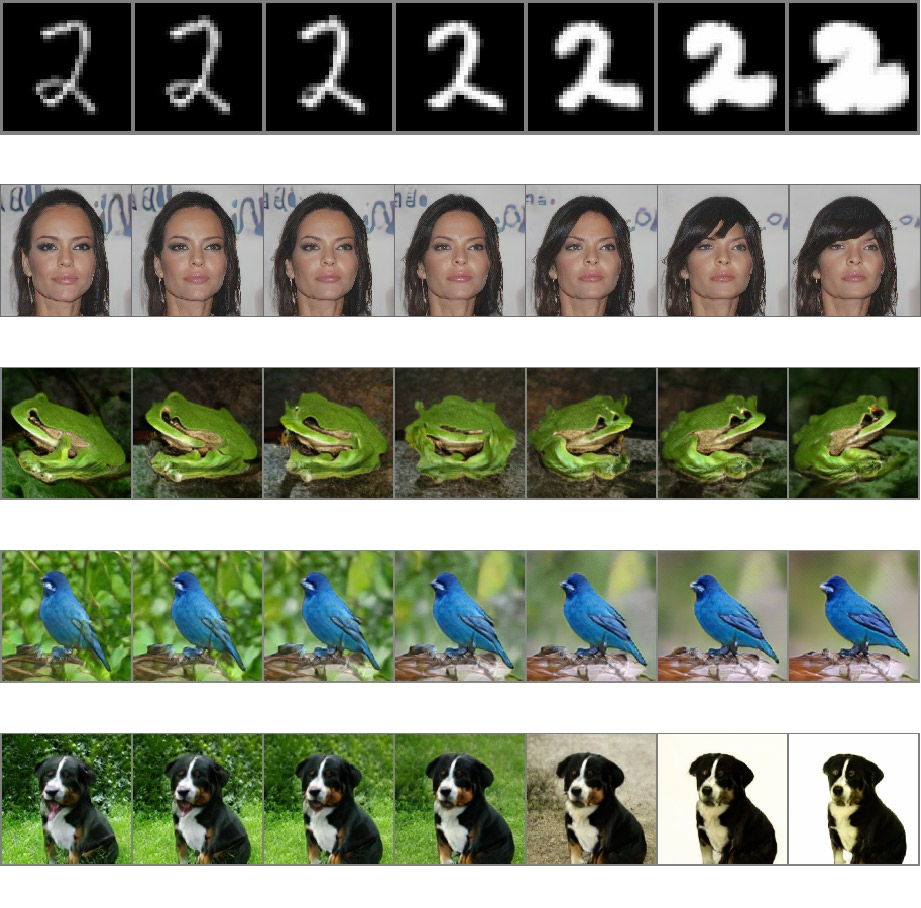
\includegraphics[width=0.85\textwidth]
        {figures/latent_space_analysis/interpretable_direction_illustration.png}
    \caption[Interpretable directions in the latent space of a generative model.]{
        Interpretable directions in the latent space of a generative model \parencite{voynov2020unsuperviseddiscoveryinterpretabledirections}.
    }
    \label{fig:interpretable_direction_illustration}
\end{figure}

A central challenge remains identifying such interpretable directions.
Most existing approaches rely on auxiliary models that encode human defined semantics, such as CLIP \parencite{haas2024discovering}, to relate latent variations to textual concepts.
Consequently, these methods inherit a limitation similar to that of probing techniques, since concept discovery depends on a pre-existing semantic framework defined by humans.

To overcome this limitation, a research direction known as unsupervised semantic discovery has emerged.
Its goal is to uncover interpretable directions in \gls{ls} without explicit semantic supervision.
In these approaches, one model applies perturbations along random directions in \gls{ls}, while a second model attempts to recognize the applied transformation.
If a stable correspondence emerges between the perturbation and its prediction, this suggests that the considered direction corresponds to a coherent \gls{cs} \parencite{voynov2020unsuperviseddiscoveryinterpretabledirections}.
In this framework, human intervention occurs only a posteriori, to verify whether the discovered directions indeed correspond to interpretable semantic variations.

Despite these advances, several challenges remain.
It appears that not all concepts encoded by \glspl{nn} are linearly identifiable in \gls{ls}.
In addition, \glspl{lr} often exhibit a phenomenon known as entanglement, illustrated in Figure~\ref{fig:entanglement_illustration}, where multiple semantic attributes are mixed within the same directions of the \gls{ls}.
For instance, in a generative face model, moving along the \enquote{glasses} direction may simultaneously modify age and gender, whereas a disentangled \gls{lr} would let each axis control a single semantic attribute while leaving the others unchanged.

This lack of separability suggests that semantic information is not cleanly organized in the \gls{ls}.
This observation motivates the \SuperpositionHypothesisName, which proposes a different view of how \glspl{nn} organize information internally.
The next section introduces this hypothesis.

\begin{figure}[t]
    \centering
    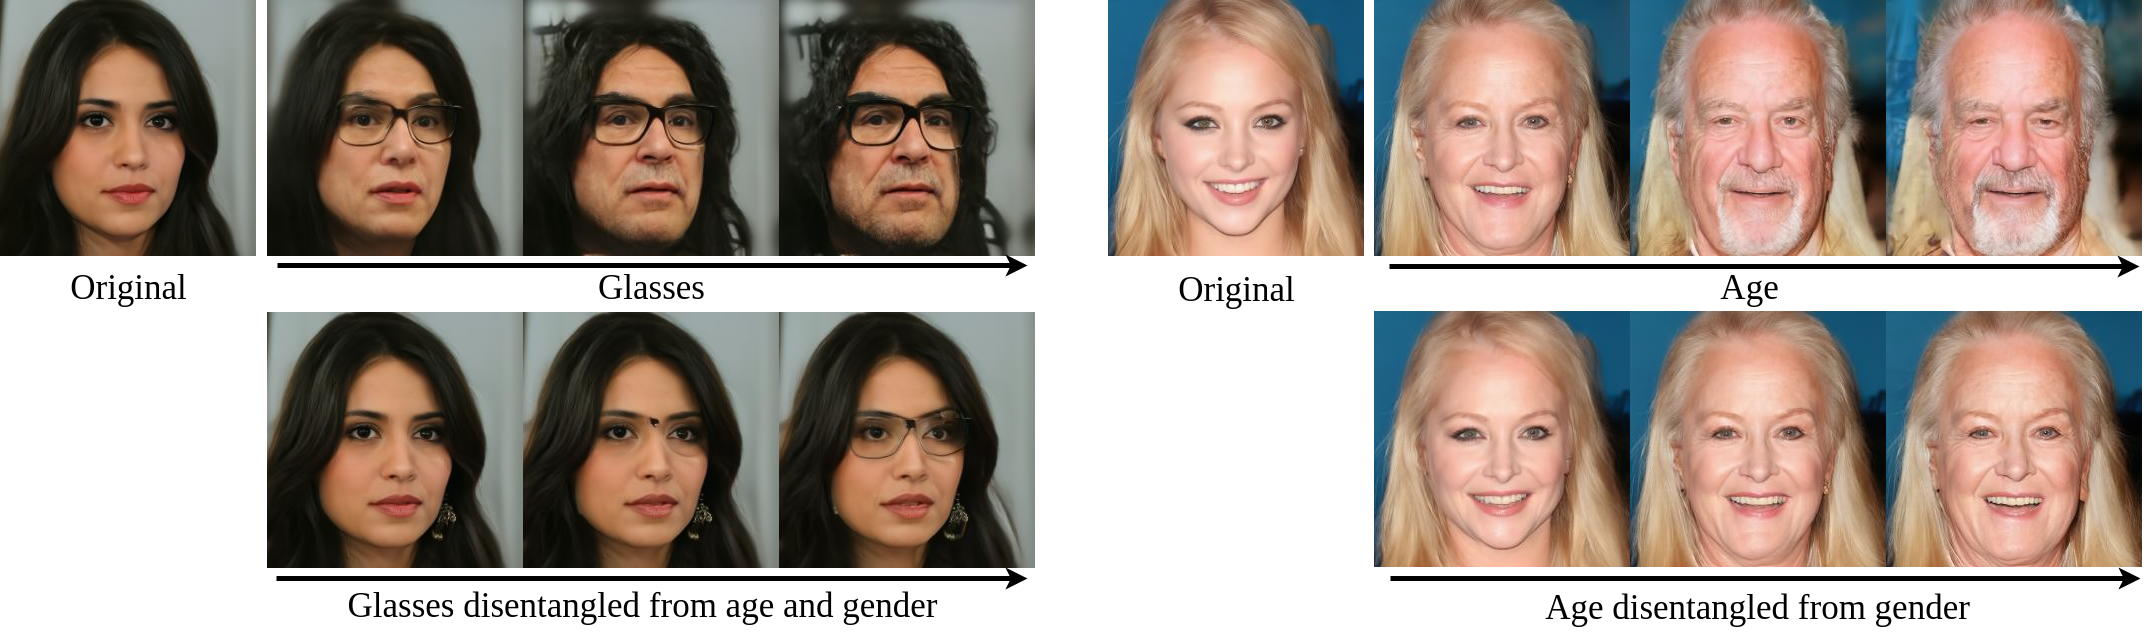
\includegraphics[width=0.85\textwidth]
        {figures/latent_space_analysis/entanglement_illustration.png}
    \caption[Entanglement in the latent space of a generative face model.]{
        Illustration of entanglement in the latent space of a generative face
        model \parencite{haas2024discovering}.
    }
    \label{fig:entanglement_illustration}
\end{figure}